\subsection{Satisfaction rate statistics generation algorithm}
\label{sec:stats}

Statistic generation is performed at different time and name prefix granularities.  
Figure~\ref{fig:stats tree} shows an overall design of the implemented statistics generation module and Pseudocodes~\ref{algo:loadstats}, \ref{algo:interest stats}, \ref{algo:prefix stats}, \ref{algo:stats} show implementation details.

\begin{figure}[htpb]
  \centering
  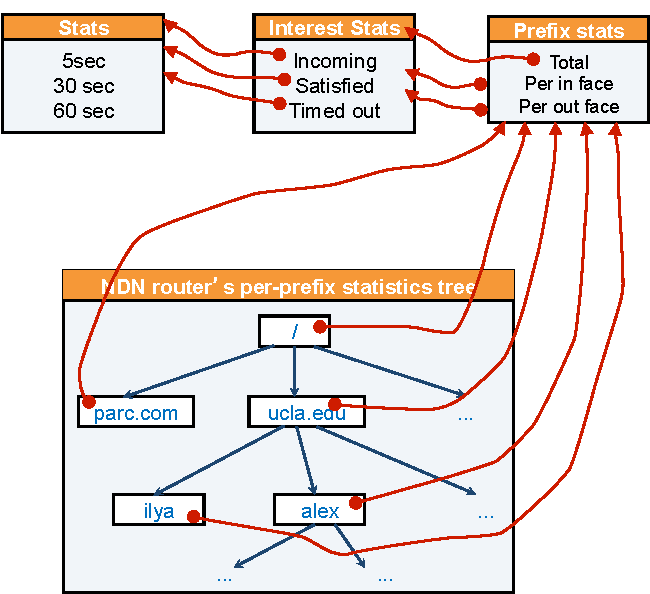
\includegraphics[scale=0.7]{figures/stats-illustration.pdf}
  \caption{Statistics tree}
  \label{fig:stats tree}
\end{figure}


A separate set of statistical information is kept for each Interest name, as well as aggregated to all Interest name prefixes, including root (``/'') prefix (per-prefix statistics tree on Figure~\ref{fig:stats tree}).

\floatname{algorithm}{Pseudocode}

%%%%%%%%%%%%%%%%%%%%%%%%%%%%%%
%%%%%%%%%%%%%%%%%%%%%%%%%%%%%%
%%%%%%%%%%%%%%%%%%%%%%%%%%%%%%

\begin{algorithm}[h]
\caption{Stats component}
\label{algo:loadstats}
\begin{algorithmic}[1]
\State $\alpha_1 \leftarrow e^{-1.0/5.0}$  \Comment{$\approx$ 5~sec average}
\State $\alpha_2 \leftarrow e^{-1.0/30.0}$ \Comment{$\approx$ 30~sec average}
\State $\alpha_3 \leftarrow e^{-1.0/60.0}$ \Comment{$\approx$ 60~sec average}
\State $avg_1 \leftarrow 0$ \, $avg_2 \leftarrow 0$ \, $avg_3 \leftarrow 0$ \, $counter \leftarrow 0$

\vspace{0.2cm}
\Function{ProcessEvent}{new Event}
\State $counter \leftarrow counter + 1$
\EndFunction

\vspace{0.2cm}
\Function{Advance}{} \Comment{Every second}
\State {} \Comment{\textit{Exponential weighted moving average smoothing}}
\State $avg_1 \leftarrow \alpha_1 \cdot avg_1 + (1 - \alpha_1) \cdot counter$ 
\State $avg_2 \leftarrow \alpha_2 \cdot avg_2 + (1 - \alpha_2) \cdot counter$
\State $avg_3 \leftarrow \alpha_3 \cdot avg_3 + (1 - \alpha_3) \cdot counter$
\State $counter \leftarrow 0$
\EndFunction
\end{algorithmic}
\end{algorithm}

%%%%%%%%%%%%%%%%%%%%%%%%%%%%%%
%%%%%%%%%%%%%%%%%%%%%%%%%%%%%%
%%%%%%%%%%%%%%%%%%%%%%%%%%%%%%

\begin{algorithm}[h]
\caption{Interest Stats component}
\label{algo:interest stats}
\begin{algorithmic}[1]
\State $I \leftarrow$ new Stats   \Comment{\# of Interests}
\State $S \leftarrow$ empty Stats \Comment{\# of satisfied Interests}
\State $U \leftarrow$ empty Stats \Comment{\# of unsatisfied Interests}

% \vspace{0.2cm}
% \Function{ProcessEvent}{new Event}
% \State $I \leftarrow counter + 1$
% \EndFunction

\vspace{0.2cm}
\Function{Combine}{other}
\State $I.counter \leftarrow other.I.counter $ 
\State $S.counter \leftarrow other.S.counter $
\State $U.counter \leftarrow other.U.counter $
\EndFunction

\vspace{0.2cm}
\Function{GetSatisfiedRatio}{}
  \For{each granularity $i$}
     \If{$I.avg_i < 0.1$}
        \State \Return $-1$ \Comment{Unknown state}
     \Else
        \State \Return $\frac{S.avg_i}{I.avg_i}$ \Comment{Interest satisfaction ratio}
     \EndIf
  \EndFor
\EndFunction

\vspace{0.2cm}
\Function{Advance}{} \Comment{Every second}
\State $I.$advance()
\State $S.$advance()
\State $U.$advance()
\EndFunction

\end{algorithmic}
\end{algorithm}

%%%%%%%%%%%%%%%%%%%%%%%%%%%%%%
%%%%%%%%%%%%%%%%%%%%%%%%%%%%%%
%%%%%%%%%%%%%%%%%%%%%%%%%%%%%%

\begin{algorithm}[h]
\caption{Prefix stats component}
\label{algo:prefix stats}
\begin{algorithmic}[1]
\State $T \leftarrow$ empty Interest Stats \Comment{Total per-prefix stats}
\For{\textbf{each} Face f}
    \State $PI[f] \leftarrow$ empty Interest Stats \Comment{per-in Face}
    \State $PO[f] \leftarrow$ empty Interest Stats \Comment{per-out Face}
\EndFor


\vspace{0.2cm}
\Function{NewPitEntry}{}
  \State $T.I.counter \leftarrow T.I.counter + 1$ %\Comment{Total \# of Interets}
\EndFunction

\vspace{0.2cm}
\Function{Incoming}{Face}
  % \State {} \Comment{per-in Face \# of Interests}
  \State $PI[Face].I.counter \leftarrow PI[Face].I.counter + 1$
\EndFunction

\vspace{0.2cm}
\Function{Outgoing}{Face}
  % \State {} \Comment{per-out Face \# of Interests}
  \State $PO[Face].I.counter \leftarrow PO[Face].I.counter + 1$
\EndFunction

\vspace{0.2cm}
\Function{Satisfy}{}
  \State $T.S.counter \leftarrow T.S.counter + 1$ %\Comment{Total \# of Interets}

  \For{\textbf{each} Face $f$}
    % \State {} \Comment{per-in Face \# of Interests}
    \State $PI[f].S.counter \leftarrow PI[f].S.counter + 1$
    % \State {} \Comment{per-out Face \# of Interests}
    \State $PO[f].S.counter \leftarrow PO[f].S.counter + 1$
  \EndFor
\EndFunction

\vspace{0.2cm}
\Function{Timeout}{}
    \State $T.U.counter \leftarrow T.U.counter + 1$ %\Comment{Total \# of Interets}

    \For{\textbf{each} Face $f$}
        % \State {} \Comment{per-in Face \# of Interests}
        \State $PI[f].U.counter \leftarrow PI[f].U.counter + 1$
        % \State {} \Comment{per-out Face \# of Interests}
        \State $PO[f].U.counter \leftarrow PO[f].U.counter + 1$
    \EndFor
\EndFunction

\vspace{0.2cm}
\Function{Combine}{other}
    \State $T.$Combine($other.T$)
    \For{\textbf{each} Face $f$}
        \State $PI[f].$Combine($other.PI[f]$)
        \State $PO[f].$Combine($other.PO[f]$)
    \EndFor
\EndFunction

\vspace{0.2cm}
\Function{Advance}{} \Comment{Every second}
\State $T.$advance()
\For{\textbf{each} Face $f$}
    \State $PI[f].$advance()
    \State $PO[f].$advance()
\EndFor

\EndFunction

\end{algorithmic}
\end{algorithm}

%%%%%%%%%%%%%%%%%%%%%%%%%%%%%%
%%%%%%%%%%%%%%%%%%%%%%%%%%%%%%
%%%%%%%%%%%%%%%%%%%%%%%%%%%%%%

\begin{algorithm}[h]
\caption{Statistics generation algorithm}
\label{algo:stats}
\begin{algorithmic}[1]

\State stats $\leftarrow$ empty tree of Prefix stats \Comment{Stats tree}

\vspace{0.2cm}
\Function{ProcessEvent}{new Interest, inFace}
  \State stats[Interest.Name].NewPitEntry()
  \State stats[Interest.Name].Incoming(inFace);
  \State stats[Interest.Name].Timeout()
\EndFunction

\vspace{0.2cm}
\Function{ProcessEvent}{Interest rejected, inFace}
  \State stats[Interest.Name].NewPitEntry()
  \State stats[Interest.Name].Incoming(inFace)
\EndFunction

\vspace{0.2cm}
\Function{ProcessEvent}{Interest forwarded, outFace}
  \State stats[Interest.Name].Outgoing(outFace)
\EndFunction

\vspace{0.2cm}
\Function{ProcessEvent}{pending Interest timeout}
  \State stats[Interest.Name].Timeout()
\EndFunction

\vspace{0.2cm}
\Function{ProcessEvent}{pending Interest satisfied}
  \State stats[Interest.Name].Satisfy()
\EndFunction

\vspace{0.2cm}
\Function{Periodic}{every second}
\For{every node, walking from children to root}
    \State $node.parent.$Combine($node$)
    \State $node.$Advance()
\EndFor
\EndFunction


\end{algorithmic}
\end{algorithm}

%%% Local Variables: 
%%% mode: latex
%%% TeX-master: "../paper"
%%% End: 
